% !TeX root = ../handout.tex

\section{Solid}

Eine mögliche Implementierung des Data Space Konzepts basiert auf Solid, welches das Ziel verfolgt, ein Fundament für offene, dezentralisierte Netzwerke für einen souveränen Datenaustausch zu schaffen.
Solid definiert dazu Protokolle für die Verwaltung und den Austausch von Daten in einer dezentralisierten Umgebung~\cite{mecklerWebLinkedData2023}.

% Solid Data Spaces
Solid Data Spaces erweitern existierende Web"=Technologien um Solid zur Bildung von Data Spaces, um eine Umgebung für sicheres Data Sharing zu erschaffen~\cite{mecklerWebLinkedData2023}.
Dafür werden Anwendungen in drei Komponenten gegliedert: die (1)~Anwendung als solches, (2)~Daten und (3)~Identität (vgl. \autoref{fig:solid-components}).

\begin{figure}[t]
    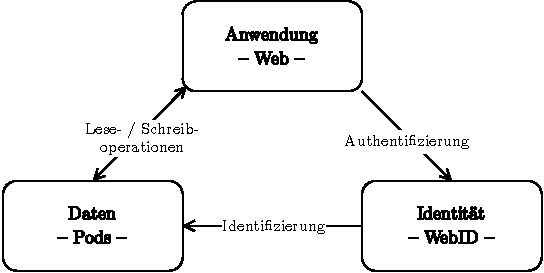
\includegraphics[width=0.7\textwidth]{./assets/solid_triangle.drawio.pdf}
    \caption{Solid-Komponenten: Anwendung, Identität und Daten}
    \label{fig:solid-components}
\end{figure}

% Komponenten
Die Identitätskomponente verifiziert die Identität eines Akteurs zur Authentifizierung für den Datenzugriff.
Die Daten und zugehörigen Zugriffsregeln werden dezentral in einem oder mehreren Datenspeichern gespeichert.
Eine Anwendung verwendet (3), um den korrekten Datenspeicher zu identifizieren und sich für den Datenzugriff zu authentifizieren.
Nach erfolgreicher Authentifizierung kann eine Anwendung die erforderlichen Daten aus (2) lesen und schreiben.
Solid definiert dabei die Protokolle zur Verwaltung von Daten und Identitäten sowie die Zugriffskontrolle.
Durch die Trennung, Standardisierung und somit Austauschbarkeit der einzelnen Komponenten, ist eine Schritt"=für"=Schritt"=Einführung möglich.
Dadurch kann die Einstiegsbarriere gering gehalten und folglich die Zugänglichkeit erhöht werden~\cite{mecklerWebLinkedData2023}.


\subsection{Datenmanagement und Datenzugriff}

Daten werden, entsprechend des Data Space Konzepts, dezentral in sog. \emph{Personal Online Data Stores} (Pods) und nicht zentral bei den Anwendungen gespeichert~\cite{mecklerWebLinkedData2023} (vgl. \autoref{fig:central-vs-decentral}).
Durch die Verwendung von Standards kann somit eine Interoperabilität auf der Daten"= statt der Anwendungsebene erzeugt werden, wodurch ein einfacher Wechsel von Anwendungen ohne aufwendige Datenmigration möglich ist.

% Datenstruktur
Da Binärdateien schlecht maschinell lesbar und somit schlecht automatisiert verarbeitbar sind, müssen zusätzliche Metadaten gespeichert werden.
Ein lesbares Format für Mensch und Maschine ist jedoch anzustreben, um eine höhere Effizienz durch Automatisierung zu ermöglichen.
Dafür wird das \emph{Resource Description Framework} (RDF) in Kombination mit \emph{Vocabularies} verwendet.
Durch eine Verknüpfung nach dem \emph{Linked Data} Ansatz entstehen strukturierte Daten mit einer automatisierbaren Semantik, welche mit verwandten Ressourcen vernetzt sind~\cite{bizerLinkedDataStory2009,mecklerWebLinkedData2023,sambraSolidPlatformDecentralized2016}.
Andere Datenstrukturen können mittels Mapping zu RDF oder als Binärdateien mit zusätzlichen Metadaten zur Speicherung der Semantik in Pods integriert werden~\cite{mecklerWebLinkedData2023,sambraSolidPlatformDecentralized2016}.

Die Daten werden in Form von \emph{Containern} gespeichert.
Diese sind an sich selbst ein RDF"=Graph, wodurch eine Hierarchie durch Verschachtelung möglich ist (vgl. Verzeichnisstruktur).
Auf jeder Ebene der Hierarchie kann eine Zugriffskontrolle über eine \emph{Access Control List} (ACL) für Ressourcen definiert werden.
Folglich können unterschiedliche Rechte pro Akteur sowie pro Ressource bzw. Container eingerichtet werden, wodurch ein feingranularer Datenschutz umsetzbar ist~\cite{mecklerWebLinkedData2023,sambraSolidPlatformDecentralized2016}.

% Lesen und Schreiben
Solid"=Anwendungen lesen und schreiben Daten direkt von und in den Pods.
Da Pods interoperabel mit den Anwendungen sind, um eine Austauschbarkeit zu gewährleisten, muss ein wohldefiniertes und möglichst einfach implementierbares Protokoll eingesetzt werden.
Solid erweitert dafür häufig bereits vorhandene RESTful"=Methoden.
% Solid verwendet dafür RESTful"=Methoden basierend auf der \emph{Linked Data Platform} (LDP).
% Es definiert bestimmte HTTP"=Operationen auf Web"=Ressourcen, wodurch alle CRUD"=Operationen abgedeckt werden.
Um eine Ressource global eindeutig zu identifizieren, ist jeder Ressource ein \emph{Uniform Resource Identifier} (URI) zugewiesen~\cite{mecklerWebLinkedData2023,sambraSolidPlatformDecentralized2016}.

% SPARQL
Mit den RESTful"=Methoden sind jedoch nur einfache Anfragen möglich.
Komplizierte Datenabfragen können optional mittels SPARQL unterstützt werden.
Um den Entwicklungsaufwand zu verringern, werden diese Operationen an den Server delegiert.
Dabei sind \emph{Local Queries}, welche nur innerhalb \emph{eines} Pods operieren, und \emph{Link Following Queries}, welche über mehrere Pods hinweg operieren, möglich.
Die tatsächliche Verteilung dieser muss dabei nicht bekannt sein~\cite{sambraSolidPlatformDecentralized2016}.


\subsection{Identität und Authentifizierung}

Um Vertrauen, Datensouveränität und Datenschutz zu gewährleisten, ist eine Authentifizierung von Akteuren notwendig.
Zum Erreichen einer Dezentralisierung ist ein globaler \emph{Identity Space} notwendig, welcher zur RDF"=basierten Daten in den Pods sowie der gewünschten Erweiterbarkeit passt und relevante Links zu den Datenspeichern liefert.
\emph{WebID} erfüllt die genannten Kriterien und wird daher in Solid verwendet~\cite{sambraSolidPlatformDecentralized2016}, kann später jedoch durch \enquote{bessere} Protokolle ersetzt werden.

Akteure besitzen eine WebID"=URI, welche ein \emph{WebID Profile Document} referenziert.
Dieses enthält wiederum Referenzen auf den Pod und die Anwendungsdaten sowie weitere Dokumente, um das Profil zu beschreiben~\cite{solidcommunitygroupSolidWebIDProfile2024}.
Das Profile Document wird bei einem \emph{Identity Provider} (meist Pod Provider) gespeichert, wodurch die Akteure die Kontrolle über ihre eigene Identität behalten~\cite{sambraSolidPlatformDecentralized2016}.

Eine Besonderheit bei Solid ist, dass sich Akteure gegenüber Anwendungen nicht authentifizieren müssen.
Eine Authentifizierung wird ggf. nur durchgeführt, um die WebID des Akteurs zu erlangen.
Anschließend wird eine Authentifizierung nur zwischen dem Browser und den relevanten Pods durchgeführt~\cite{sambraSolidPlatformDecentralized2016}.

Durch die Möglichkeit, Identitäten über mehrere Seiten hinweg zu verknüpfen, entsteht ein \emph{Web of Trust}.
Dies ermöglicht es, Authentifizierungsentscheidungen ad-hoc basierend auf den Eigenschaften der Akteure, wie bspw. den Beziehungen zu anderen Akteuren, zu treffen~\cite{sambraSolidPlatformDecentralized2016}.
Auf dieser Basis kann entschieden werden, wem vertraut werden kann, mit wem ein vertrauenswürdiger Datenaustausch möglich ist und ob in den Wahrheitsgehalt der geteilten Daten vertraut werden kann.
Somit wird ein großes Hindernis des Data Sharings direkt adressiert.


\subsection{Erweiterung: Wertschöpfungsketten}

Eine automatisierte Datenübertragung ist essenziell für Partner in einer Wertschöpfungskette, ist jedoch an weitere Anforderungen geknüpft.
So müssen bspw. rechtliche Rahmenbedingungen garantiert und nachvollziehbar eingehalten werden.
Solid bietet dafür bereits eine Grundlage, ist aber noch nicht ausreichend.
Weitere Methoden sind notwendig, um \emph{Constraints} für das Data Sharing zu etablieren~\cite{bothSolidBasedB2BData2025}.

Zum einen kann über Metadaten ein \emph{Data Processing Purpose} $P$ angegeben werden, welche die minimal möglichen und notwendigen Rechte beschreibt.
Die Weitergabe von Daten soll nur unter mindestens genauso starken Restriktionen erlaubt sein.
Dafür führt \cite{bothSolidBasedB2BData2025} eine \emph{Purpose}"=Klasse ein, welche weitergegeben werden muss~\cite{bothSolidBasedB2BData2025}.

Andererseits soll die ursprüngliche Quelle bei der Weitergabe von Daten versteckt werden.
Um eine spätere Nachvollziehbarkeit zu garantieren, soll jedoch angegeben werden, dass die Zugriffsrechte und weitergegebenen Daten auf einer Freigabe durch eine Drittpartei basieren.
Dies wird durch eine \emph{Facade}"=Klasse umgesetzt, welche den ursprünglichen Data Provider versteckt~\cite{bothSolidBasedB2BData2025}. Ein Beispiel ist in \autoref{fig:example-data-donation} dargestellt.

Diese Erweiterung zeigt die Möglichkeiten und Notwendigkeit der Erweiterbarkeit von Solid.
Sie dient als weiterer Schritt in Richtung Wertschöpfungsketten unter der Berücksichtigung des Schutzes von Daten und Geschäftsgeheimnissen.
Allerdings ist weitere Forschung notwendig, um die verwendeten Methoden zu validieren, um vollständig automatisierbare Prozesse in der Breite zu etablieren~\cite{bothSolidBasedB2BData2025}.
